% -*- mode: latex; mode: flyspell; ispell-local-dictionary: "en_US"; coding: utf-8; fill-column: 80 -*-

\documentclass{article}

\usepackage[utf8]{inputenc}
\usepackage[english]{babel}

\usepackage{amsmath,amsfonts,amssymb}
\usepackage{fullpage}
\usepackage{verbatim}

\usepackage{tikz,pgfplots}

\pgfplotsset{
  width=150mm,height=100mm,
  major grid style={thin,dotted,color=black!50},
  minor grid style={thin,dotted,color=black!50},
  grid,
  every axis/.append style={
    line width=0.5pt,
    tick style={
      line cap=round,
      thin,
      major tick length=4pt,
      minor tick length=2pt,
    },
  },
  legend cell align=left,
  legend pos=north west,
}

%%%%%%%%%%%%%%%%%%%%%%%%%%%%%%%%%%%%%%%%%%%%%%%%%%%%%%%%%%%%%%%%%%%%%%%%%%%%%%%%

\begin{document}

\title{Laufzeit binäre Suche vs. Mphf-Hashmap}
\author{Tim Tannert}
\maketitle

% IMPORT-DATA stats output/mphf_vs_bs.txt



\begin{center}
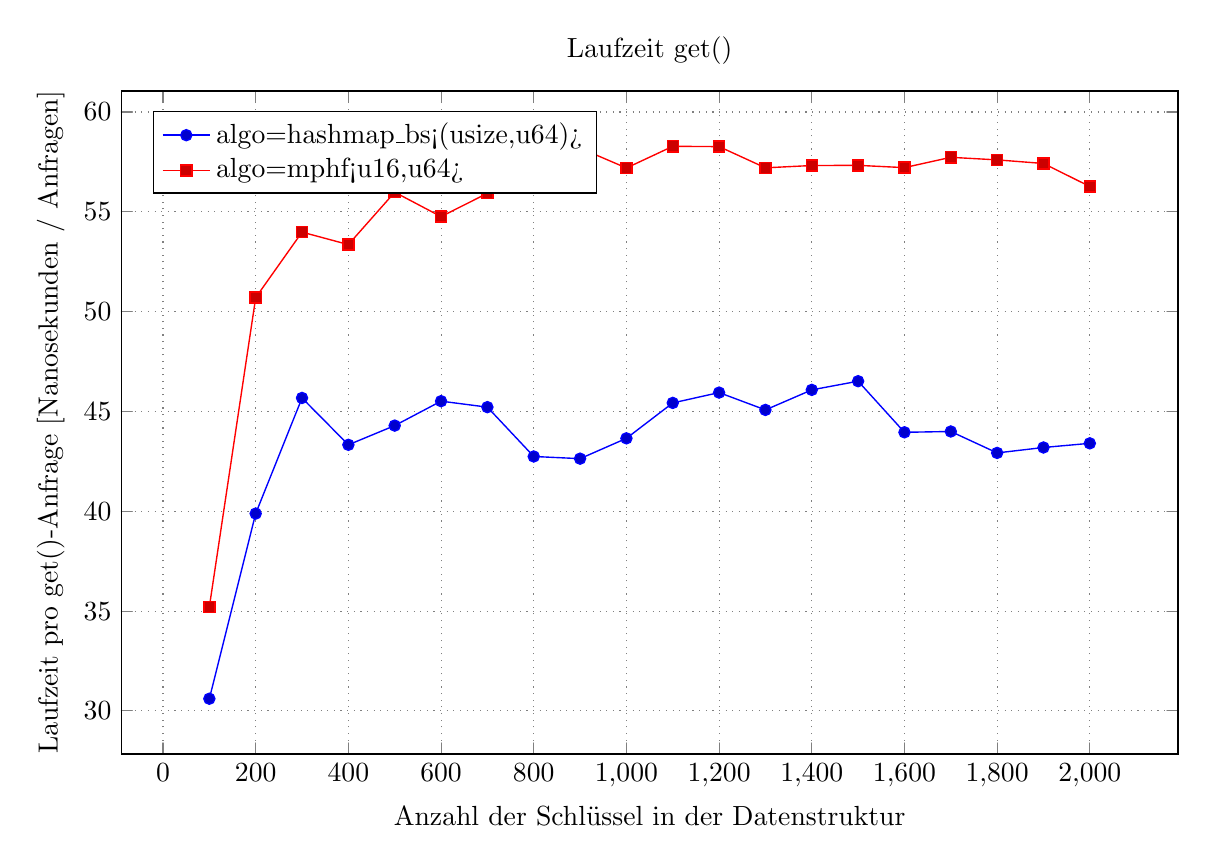
\begin{tikzpicture}
  \begin{axis}[
    title={Laufzeit get()},
    xlabel={Anzahl der Schlüssel in der Datenstruktur},
    ylabel={Laufzeit pro get()-Anfrage [Nanosekunden / Anfragen]},
    ]

    %% MULTIPLOT(algo) SELECT size AS x, MEDIAN(time_per_anfrage) AS y, MULTIPLOT
    %% FROM stats WHERE x % 100 == 0  GROUP BY MULTIPLOT,x ORDER BY MULTIPLOT,x
    \addplot coordinates { (100,30.61) (200,39.885) (300,45.6767) (400,43.32875) (500,44.292) (600,45.5158) (700,45.2157) (800,42.745) (900,42.6356) (1000,43.6535) (1100,45.4282) (1200,45.9454) (1300,45.0773) (1400,46.0814) (1500,46.5157) (1600,43.9559) (1700,43.9971) (1800,42.9233) (1900,43.1953) (2000,43.40375) };
    \addlegendentry{algo=hashmap\_bs<(usize,u64)>};
    \addplot coordinates { (100,35.21) (200,50.7025) (300,53.9833) (400,53.35875) (500,55.983) (600,54.76) (700,55.93) (800,57.7156) (900,58.1933) (1000,57.1955) (1100,58.2814) (1200,58.2675) (1300,57.2046) (1400,57.32) (1500,57.3283) (1600,57.2144) (1700,57.7312) (1800,57.6025) (1900,57.4221) (2000,56.27) };
    \addlegendentry{algo=mphf<u16,u64>};
    



  \end{axis}
\end{tikzpicture}
\end{center}





\end{document}
%%%%%%%%%%%%%%%%%%%%%%%%%%%%%%%%%%%%%%%%%%%%%%%%%%%%%%%%%%%%%%%%%%%%%%%%%%%%%%%%
